\section{Remote Visual Display (RVD) Protocol}

The RVD protocol is used to communicate mouse input, keyboard input, frame data, and clipboard data between the
Host and the Client.\\

All messages MUST occur over the transport listed.\\

With the exception of the \emph{Handshake} messages, all RVD messages' first byte contain a number to indicate
the message type. \\

A \emph{sequence-number} is an incrementing 32-bit counter each UDP message sent, separate for Host and Client. All
messages sent over UDP MUST begin with a 4 bytes \emph{sequence-number}. \emph{sequence-number} is initialized
to 0 and increments once for every UDP message sent by the respective Peer. Therefore each RVD UDP message looks
like:

\begin{center}
    \begin{tabular}{|c|c|}
        \hline
        \textbf{Bytes} & \textbf{Name}   \\
        \hline
        4              & sequence-number \\
        \hline
        variable       & RVD message     \\
        \hline
    \end{tabular}
\end{center}

\subsection{Combining Messages}

In some situations, such as when a large screen change occurs or when the screen is first sent to the client,
large amounts of \emph{FrameData}'s may need to be sent in quick succession. Often individual \emph{FrameData}'s
will be much smaller than the MTU. Similar to TCP's Nagle algorithm, multiple UDP messages can be combined into a
single UDP packet as long as the total size is remains less than the MTU. Each message directly follows the
previous message with the first message directly following the sequence number. Only one \emph{sequence-number}
is used:

\begin{center}
    \begin{tabular}{|c|c|}
        \hline
        \textbf{Bytes} & \textbf{Name}   \\
        \hline
        4              & sequence-number \\
        \hline
        variable       & RVD message 1   \\
        \hline
        variable       & RVD message 2   \\
        \hline
        \hline
        variable       & etc.            \\
        \hline
    \end{tabular}
\end{center}

\subsection{Definitions}

\begin{itemize}
    \item Host - A peer with an ID that wants to share their screen to the Client
    \item Client - A peer that wants to view and maybe control the Host's screen
    \item Display - A rectangular visual region that is shared by a Host to a Client. May or may not be
    \item \emph{Controllable}.
    \item Controllable - A \emph{Display} that accepts keyboard and mouse input.
\end{itemize}

\subsection{Handshake}

\subsubsection{ProtocolVersion - TCP}
Handshaking begins by the Host sending the client a \emph{ProtocolVersion} message. This lets the Client know the
verison supported by the Host.\\

The \emph{ProtocolVersion} message consists of 11 bytes interpreted as a string of ASCII characters in the format
"RVD xxx.yyy" where xxx and yyy are the major and minor version numbers, padded with zeros.

\begin{center}
    Host \textrightarrow\ Client\\
    \begin{tabular}{|c|c|c|}
        \hline
        \textbf{Bytes} & \textbf{Name} & \textbf{Value}           \\
        \hline
        11             & version       & ``\texttt{RVD 001.000}'' \\
        \hline
    \end{tabular}
\end{center}

The Client replies back either \texttt{0} to indicate the version is not acceptable and that the handshake has
failed or \texttt{1} if the version is acceptable to the Client and the handshake as succeeded. If 0 is sent, all
communication MUST cease and an error SHOULD be displayed to user. A \emph{SessionEnd} message should be sent by
the Client. % TODO hyper

\begin{center}
    Client \textrightarrow\ Host\\
    \begin{tabular}{|c|c|c|}
        \hline
        \textbf{Bytes} & \textbf{Name} & \textbf{Value} \\
        \hline
        1              & ok            & 0 or 1         \\
        \hline
    \end{tabular}
\end{center}

\subsubsection{Initialization}

Once the handshake has succeeded the Host responds with a \emph{DisplayChange} message.

\subsection{Control messages}
Control messages are messages that instruct client about changes regarding the Host.

\subsubsection{DisplayChange - TCP}
A \emph{DisplayChange} message informs the client about the available \emph{Display}s. RVD supports up to 255
displays.

\begin{center}
    Host \textrightarrow\ Client\\
    \begin{tabular}{|c|c|c|}
        \hline
        \textbf{Bytes} & \textbf{Name}        & \textbf{Value}            \\
        \hline
        1              & type                 & 1                         \\
        \hline
        1              & clipboard-readable   & 0 or 1                    \\
        \hline
        1              & number-of-displays   & 1 - 255                   \\
        \hline
        variable       & displays-information & \emph{DisplayInformation} \\
        \hline
    \end{tabular}
\end{center}

Each \emph{Display} has an associated \emph{DisplayInformation}. \emph{displays-information} contains
\emph{number-of-displays} \emph{DisplayInformation}'s. A \emph{DisplayInformation} is defined below:

\begin{center}
    \begin{tabular}{|c|c|c|}
        \hline
        \textbf{Bytes}     & \textbf{Name} & \textbf{Description}                                 \\
        \hline
        1                  & display-id    &                                                      \\
        \hline
        2                  & width         & number of pixels of the width of this display        \\
        \hline
        2                  & height        & number of pixels of the width of this display        \\
        \hline
        2                  & cell-width    & number of pixels of the height of a cell in the grid \\
        \hline
        2                  & cell-height   & number of pixels of the height of a cell in the grid \\
        \hline
        1                  & access        & defined below                                        \\
        \hline
        1                  & name-length   & length of the \emph{display-name} in bytes           \\
        \hline
        \emph{name-length} & display-name  & the display name (UTF-8)                             \\
        \hline
    \end{tabular}
\end{center}

\textbf{Restrictions:}

\begin{itemize}
    \item \emph{cell-width} MUST be less than \emph{width}. \emph{cell-height} must be less than \emph{height}.\\
    % // TODO define more restrictions %
    \item The \emph{access} byte defines what type of access is available for the display. The bits of the
    \emph{access} byte are described below in little endian.
\end{itemize}


\begin{center}
    \begin{tabular}{|c|c|}
        \hline
        \textbf{Bit} & \textbf{Name}                               \\
        \hline
        0            & Flush                                       \\
        \hline
        1            & \emph{Controllable}                         \\
        \hline
        2            & \multirow{6}{10em}{Reserved for future use} \\
        3            &                                             \\
        4            &                                             \\
        5            &                                             \\
        6            &                                             \\
        7            &                                             \\
        \hline
    \end{tabular}
\end{center}

If the \emph{Controllable} bit is 1 and the \emph{clipboard-readable} byte is set to 1, then the clipboard is
writable. The \emph{Controllable} bit SHOULD be consistent throughout all displays.\\

The \emph{Flush} bit indicates whether this display has changed, specifically if this \emph{display-id} refers to
a different \emph{Display} than the same \emph{display-id} did in the previous \emph{DisplayChange} message. In
initialization, this MUST always be 1 (as there is no previous \emph{DisplayChange}). If the display hasn't
changed (0) then the frame data may be maintained. If \emph{Flush} is 0, \emph{width}, \emph{height} MUST remain
the same as the previous \emph{DisplayChange} specified for the \emph{display-id}.\\


Display cell numbering is right to left, up to down, 0 indexed as seen below. If $\text{cell-width}\ \%\
\text{width} > 0$ the right column's width will be $\text{width}\ \%\ \text{cell-width}$. If $\text{height}\
\%\ \text{cell-height} > 0$ the bottom row's height will be $\text{height}\ \%\ \text{cell-height}$.

\begin{center}
    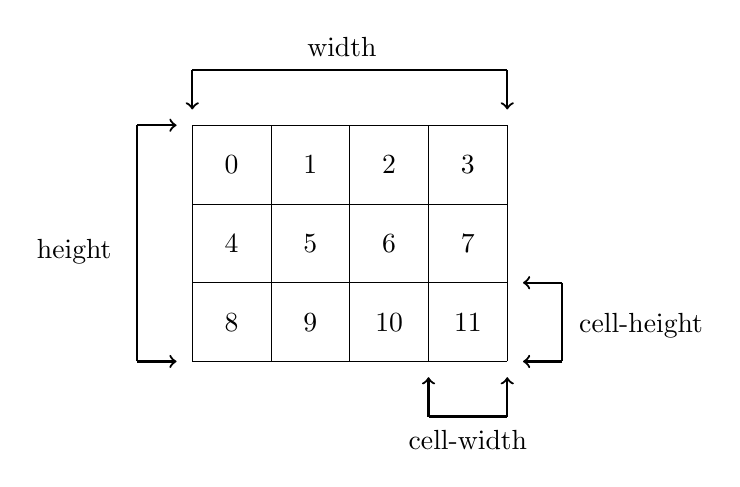
\begin{tikzpicture}
        \draw[step=1cm,black,very thin] (0,0) grid (4,3);
        \draw[thick,->] (-0.7,3) -- (-0.2,3);
        \draw[thick] (-0.7,3) -- (-0.7,0);
        \draw[thick,->] (-0.7,0) -- (-0.2,0);
        \draw (-1.5,1.4) node{height};

        \draw[thick,->] (0,3.7) -- (0,3.2);
        \draw[thick] (0,3.7) -- (4,3.7);
        \draw[thick,->] (4,3.7) -- (4,3.2);
        \draw (1.9,4) node{width};

        \draw[thick,->] (4.7,1) -- (4.2,1);
        \draw[thick] (4.7,1) -- (4.7,0);
        \draw[thick,->] (4.7,0) -- (4.2,0);
        \draw (5.7,0.45) node{cell-height};

        \draw[thick,->] (3,-0.7) -- (3,-0.2);
        \draw[thick] (3,-0.7) -- (4,-0.7);
        \draw[thick,->] (4,-0.7) -- (4,-0.2);
        \draw (3.5, -1) node{cell-width};

        \draw (0.5, 2.5) node{0};
        \draw (1.5, 2.5) node{1};
        \draw (2.5, 2.5) node{2};
        \draw (3.5, 2.5) node{3};

        \draw (0.5, 1.5) node{4};
        \draw (1.5, 1.5) node{5};
        \draw (2.5, 1.5) node{6};
        \draw (3.5, 1.5) node{7};

        \draw (0.5, 0.5) node{8};
        \draw (1.5, 0.5) node{9};
        \draw (2.5, 0.5) node{10};
        \draw (3.5, 0.5) node{11};
    \end{tikzpicture}
\end{center}

\subsubsection{DisplayChangeReceived - TCP}

The \emph{DisplayChangeReceived} message is sent in reply after receiving a \emph{DisplayChange} message. It
indicates to the Host they may start sending \emph{FrameData} referencing the new \emph{DisplayInformation} in
the most recent \emph{DisplayChange}.

\begin{center}
    Client \textrightarrow\ Host\\
    \begin{tabular}{|c|c|c|}
        \hline
        \textbf{Bytes} & \textbf{Name} & \textbf{Value} \\
        \hline
        1              & type          & 2              \\
        \hline
    \end{tabular}
\end{center}

\subsubsection{MouseLocation - TCP/UDP}

The \emph{MouseLocation} message send information about where the mouse is currently on the screen.
The Host sends this information periodically throughout the session.
The Host SHOULD send a \emph{MouseLocation} update when mouse input is received from the Host's system or in
reply when it receives a \emph{MouseInput}.

\begin{center}
    Host \textrightarrow\ Client\\
    \begin{tabular}{|c|c|c|c|}
        \hline
        \textbf{Bytes} & \textbf{Name} & \textbf{Value} & \textbf{Description}      \\
        \hline
        3              & type          & 3              &                           \\
        \hline
        1              & display-id    & 0-255          &                           \\
        \hline
        2              & x-location    &                & x coordinate of the mouse \\
        \hline
        2              & y-location    &                & y coordinate of the mouse \\
        \hline
    \end{tabular}
\end{center}

\subsection{Input}

Input messages (including \emph{MouseLocation}) may be sent over TCP or UDP. TCP is preferred in most situations.
However, in situations where speed is prioritized over the guarantees TCP provides (such as gaming), UDP can be
used.

\subsubsection{MouseInput - TCP/UDP}

\begin{center}
    Client \textrightarrow\ Host\\
    \begin{tabular}{|c|c|c|c|}
        \hline
        \textbf{Bytes} & \textbf{Name} & \textbf{Value} & \textbf{Description}      \\
        \hline
        1              & type          & 4              &                           \\
        \hline
        1              & display-id    & 0-255          &                           \\
        \hline
        2              & x-position    &                & x coordinate of the mouse \\
        \hline
        2              & y-position    &                & y coordinate of the mouse \\
        \hline
        1              & button-mask   &                & described below           \\
        \hline
    \end{tabular}
\end{center}

%  https://github.com/rfbproto/rfbproto/blob/master/rfbproto.rst#pointerevent %
Indicates either pointer movement or a pointer button press or release. The pointer is now at (x-position,
y-position), and the current state of buttons 1 to 8 are represented by bits 0 to 7 of button-mask respectively,
0 meaning up, 1 meaning down (pressed).\\

On a conventional mouse, buttons 1, 2 and 3 correspond to the left, middle and right buttons on the mouse. On a
wheel mouse, each step of the wheel is represented by a press and release of a certain button. Button 4 means up,
button 5 means down, button 6 means left and button 7 means right.

\subsubsection{KeyInput - TCP/UDP}

The \emph{KeyInput} event sends key presses or releases.

\begin{center}
    Client \textrightarrow\ Host\\
    \begin{tabular}{|c|c|c|c|}
        \hline
        \textbf{Bytes} & \textbf{Name} & \textbf{Value} & \textbf{Description}                                 \\
        \hline
        1              & type          & 5              &                                                      \\
        \hline
        1              & down-flag     & 0 or 1         & indicates whether the key is now pressed or released \\
        \hline
        4              & key           &                & "keysym"                                             \\
        \hline
    \end{tabular}
\end{center}

Details can be found at the \href{https://github.com/rfbproto/rfbproto/blob/master/rfbproto.rst#keyevent}{RFB Spec}

\subsection{Clipboard} % // TODO this needs to be worked on

\subsubsection{ClipboardTypeRequest - TCP}

Used to request clipboard types the Host supports.

\begin{center}
    Client \textrightarrow\ Host\\
    \begin{tabular}{|c|c|c|}
        \hline
        \textbf{Bytes} & \textbf{Name} & \textbf{Value} \\
        \hline
        1              & type          & 6              \\
        \hline
    \end{tabular}
\end{center}

\subsubsection{ClipboardTypeResponse - TCP}

Response to the \emph{ClipboardTypeRequest}

\begin{center}
    Host \textrightarrow\ Client\\
    \begin{tabular}{|c|c|c|c|}
        \hline
        \textbf{Bytes} & \textbf{Name}             & \textbf{Value} & \textbf{Description} \\
        \hline
        1              & type                      & 7              &                      \\
        \hline
        1              & number-of-clipboard-types & 0-255          &                      \\
        \hline
        variable       & data (variable bytes)     &                & described below      \\
        \hline
    \end{tabular}
\end{center}

\emph{number-of-clipboard-types} is always 0 if \emph{clipboard-readable} is 0.\\

\emph{data} contains \emph{number-of-clipboard-types} \emph{ClipboardType}s. \emph{ClipboardType} is defined below.

\begin{center}
    \begin{tabular}{|c|c|c|c|}
        \hline
        \textbf{Bytes}     & \textbf{Name} & \textbf{Value} & \textbf{Description} \\
        \hline
        1                  & type-length   & 1-255          &                      \\
        \hline
        \emph{type-length} & type-name     &                & type name in ASCII   \\
        \hline
    \end{tabular}
\end{center}

\subsubsection{CopyRequest - TCP}

This is a request for a keyboard contents. It can be made by either the Client or the Host.

\begin{center}
    Client $\leftrightarrow$ Host\\
    \begin{tabular}{|c|c|c|c|}
        \hline
        \textbf{Bytes}     & \textbf{Name} & \textbf{Value} & \textbf{Description} \\
        \hline
        1                  & type          & 8              &                      \\
        \hline
        1                  & type-length   & 1-255          &                      \\
        \hline
        \emph{type-length} & type-name     &                & type name in ASCII   \\
        \hline
    \end{tabular}
\end{center}

\subsubsection{CopyResponse - TCP}

\emph{CopyResponse} message is a response to a \emph{CopyRequest}.

\begin{center}
    Client $\leftrightarrow$ Host\\
    \begin{tabular}{|c|c|c|c|}
        \hline
        \textbf{Bytes}        & \textbf{Name} & \textbf{Value} & \textbf{Description} \\
        \hline
        1                     & type          & 9              &                      \\
        \hline
        1                     & accepted      & 0 or 1         &                      \\
        \hline
        \multicolumn{4}{|c|}{\textbf{Below only if \emph{accepted} is 1} } \\
        \hline
        1                     & type-length   & 1-255          &                      \\
        \hline
        \emph{type-length}    & type-name     &                & type name in ASCII   \\
        \hline
        3 & content-length & & the length of the content  (maximum $2^{24}$
        bytes or ~16MB ) \\
        \hline
        \emph{content-length} & data          &                & zlib'ed raw data     \\
        \hline
    \end{tabular}
\end{center}



\emph{accepted} indicates whether the \emph{CopyRequest} was accepted. If 0, the rest of the message MUST not exist.
If \emph{clipboard-readable} is 0, \emph{accepted} is always 0. A Client or Host may send this message without a
request.
If a \emph{CopyResponse} is unsolicited, then \emph{accepted} MUST be 1.\\

\emph{data} is zlib compressed.

\subsubsection{A note on Pasting}

There is a no paste message. To paste data an unsolicited \emph{CopyResponse} may be sent and then the keyboard
shortcut (ctrl+v or cmd+v) should be sent via the \emph{KeyboardMessage}

\subsection{FrameData - UDP}
The \emph{FrameData} message contains an update of a particular cell on a particular \emph{Display}.

\begin{center}
    Host \textrightarrow Client\\
    \begin{tabular}{|c|c|c|}
        \hline
        \textbf{Bytes} & \textbf{Name} & \textbf{Value} \\
        \hline
        1              & type          & 10             \\
        \hline
        4              & frame-number  &                \\
        \hline
        1              & display-id    & 0-255          \\
        \hline
        2              & cell-number   &                \\
        \hline
        2              & size          &                \\
        \hline
        \emph{size}    & data          &                \\
        \hline
    \end{tabular}
\end{center}

\emph{frame-number} is a 32 bit counter, initialized with 0 at the begining of the protocol, and incremented once
from \emph{FrameData} message sent.

\emph{data} contains jpeg pixel data of the updated cell.

\subsection{Congestion}

When sending messages over a network the network may become congested to avoid congesting the network further RVD
implements a congestion detection and congestion control mechanism. RVD uses Additive increase/multiplicative
decrease or AIMD to control the \emph{OutputMaximum} which is the maximum messages allowed per
\emph{CongestionWindow}.